\documentclass[12pt,a4paper]{article}
\usepackage{amsmath,amscd,amsbsy,amssymb,latexsym,url,bm,amsthm}
\usepackage{epsfig,graphicx,subfigure}
\usepackage{enumitem,balance}
\usepackage{wrapfig}
\usepackage{mathrsfs,euscript}
\usepackage[usenames]{xcolor}
\usepackage{hyperref}
\usepackage[vlined,ruled,linesnumbered]{algorithm2e}
\hypersetup{colorlinks=true,linkcolor=black}

\newtheorem{theorem}{Theorem}
\newtheorem{lemma}[theorem]{Lemma}
\newtheorem{proposition}[theorem]{Proposition}
\newtheorem{corollary}[theorem]{Corollary}
\newtheorem{exercise}{Exercise}
\newtheorem*{solution}{Solution}
\newtheorem{definition}{Definition}
\theoremstyle{definition}

\renewcommand{\thefootnote}{\fnsymbol{footnote}}

\newcommand{\postscript}[2]
 {\setlength{\epsfxsize}{#2\hsize}
  \centerline{\epsfbox{#1}}}

\renewcommand{\baselinestretch}{1.0}

\setlength{\oddsidemargin}{-0.365in}
\setlength{\evensidemargin}{-0.365in}
\setlength{\topmargin}{-0.3in}
\setlength{\headheight}{0in}
\setlength{\headsep}{0in}
\setlength{\textheight}{10.1in}
\setlength{\textwidth}{7in}
\makeatletter \renewenvironment{proof}[1][Proof] {\par\pushQED{\qed}\normalfont\topsep6\p@\@plus6\p@\relax\trivlist\item[\hskip\labelsep\bfseries#1\@addpunct{.}]\ignorespaces}{\popQED\endtrivlist\@endpefalse} \makeatother
\makeatletter
\renewenvironment{solution}[1][Solution] {\par\pushQED{\qed}\normalfont\topsep6\p@\@plus6\p@\relax\trivlist\item[\hskip\labelsep\bfseries#1\@addpunct{.}]\ignorespaces}{\popQED\endtrivlist\@endpefalse} \makeatother

\begin{document}
\noindent

%========================================================================
\noindent\framebox[\linewidth]{\shortstack[c]{
\Large{\textbf{Lab03-Greedy Strategy}}\vspace{1mm}\\
CS214-Algorithm and Complexity, Xiaofeng Gao, Spring 2019.}}


\begin{center}
\footnotesize{\color{red}$*$ If there is any problem, please contact TA Mingran Peng.}\par
% Please write down your name, student id and email.
\footnotesize{\color{blue}$*$ Name: KylinChen  \quad Student ID: 517030910155 \quad Email: k1017856853@icloud.com }
\end{center}
\begin{enumerate}
    \item
    Suppose there is a street with length $n$, described by an array $A[1...n]$ where $A[i]=1$ means that there is a house at position $i$ and $A[i]=0$ means position $i$ is vacant.\par
	According to some law, every house must be protected by fire hydrant. If a fire hydrant is placed at position $i$, then all houses at postion $i-1,i,i+1$ will be considered protected. Note that hydrants can be placed at the same place with a house.\par
	Using what you learnt in class, please design an algorithm that computes the minimum number of hydrants needed to protect all houses. You need to write pseudo code, analyze the time complexity,  and prove its correctness.\par
    \begin{solution}\item
    \renewcommand{\qedsymbol}{}
    \textbf{Algorithm Description:}
    \item
    \begin{itemize}
    \item [1)] First, we put a \textbf{flag} at street head, Then go to the next 2) step.
    \item [2)] If the \textbf{flag} points a house, go to 3) step. If the \textbf{flag} doesn't point a house, go to 4) step.
    \item [3)] Put a hydrant in the next adjacent position, which can cover this house. Then move the \textbf{flag} to next three position, which can't be covered by previous hydrants. Finally, we can go to 5) step.
    \item [4)] Now that we didn't find the house, we move the \textbf{flag} to next one position. Finally, we can go to 5) step.
    \item [5)] If the position is out of range, end it to get all the hydrants. Otherwise, we can go to 2) step.
    \end{itemize}\item
    This algorithm can described by pseudo code as follows. Algorithm.~\ref{ALG1} is to find the greedy set of all hydrants position, while Algorithm.~\ref{ALG2} is to find the greedy optimal number of hydrants.
    \item
    \textbf{Pseudo Code:}
    \item
        \begin{minipage}[t]{0.9\textwidth}
        \begin{algorithm}[H]
        \KwIn{An array $A[1 \cdots n]$}
        \KwOut{Set $B$ contains all the optimal locations of hydrants}
        \BlankLine
        \caption{Greedy-Selection}
        \label{ALG1}
        \BlankLine
	    $B\leftarrow \emptyset$\;
	    $i\ \leftarrow 1$\;
	    \While{$i \leq n$}{
	    \If{$A[i]==1$}{
	         $B\leftarrow B\cup \{i+1\}$\;
	         $i\leftarrow i+3$\;
	    }
	    \Else{
	        $i\leftarrow i+1$\;
	    }
	    }

        \end{algorithm}
        \end{minipage}
        \hfill

        \begin{minipage}[t]{0.9\textwidth}
        \begin{algorithm}[H]
        \KwIn{An array $A[1 \cdots n]$}
        \KwOut{Number $C$, which describe the number of hydrants}
        \BlankLine
        \caption{Greedy-Count}
        \label{ALG2}
        \BlankLine
	    $C\leftarrow 0$\;
	    $i\ \leftarrow 1$\;
	    \While{$i \leq n$}{
	    \If{$A[i]==1$}{
	         $C\leftarrow C+1$\;
	         $i\leftarrow i+3$\;
	    }
	    \Else{
	        $i\leftarrow i+1$\;
	    }
	    }

        \end{algorithm}
        \end{minipage}
        \hfill
    \item\item\textbf{Complexity Analysis:}
    \item
    \begin{itemize}
    	\item [] Let input array = $A$ and $n=$ $A's$ length.
    	\item If the input array $A$ is 0-array, the \textbf{while-loop} will take maximum $O(n)$ time. 
    	\item If the input array $A$ satisfies restrictions:$A[1+3 \times k]=1\ (k \in \mathbb{N})$, The \textbf{while-loop} will take minimun $O(\frac{n}{3})=O(n)$ time.
    \end{itemize}
    Thus, Greedy-Selection algorithm takes $O(n)$ time.\item
    \textbf{Correctness Proof:}\item
    \begin{itemize}
    	\item [] \textbf{Claim.} The Greedy-Selection algorithm is optimal.\par (If there exsits more than one optimal solution, greedy solution has same number of hydrants with other optimal solution)
    	\item [] \textbf{Proof.} 
    	Define $G$ is Greed-Selection, $O$ is Optimized-Selection. Assume before k-th selection, $G$ and $O$ have same positions chosen. In the k-th selection, $G$ select position $e$ while $O$ select position $f$.
    	\begin{itemize}
    		\item [] $Invariant 1:$ There exists an optimal selection $O$ that makes $G$ and $O$ have same position choice through the k-th selection.
    		\item [] $Invariant 2:$ There exists an optimal selection $O$ that makes $G$ and $O$ have different position choice at the k-th selection, but for k+1 selction, it make no sense for k-th selection's homogeny.
    		\item  \textbf{case 1:} If $e=f$, it means $O$ and $G$ select same position, which satisfies $Invariant 1$.
    		\begin{figure}[htbp]
                \centering
                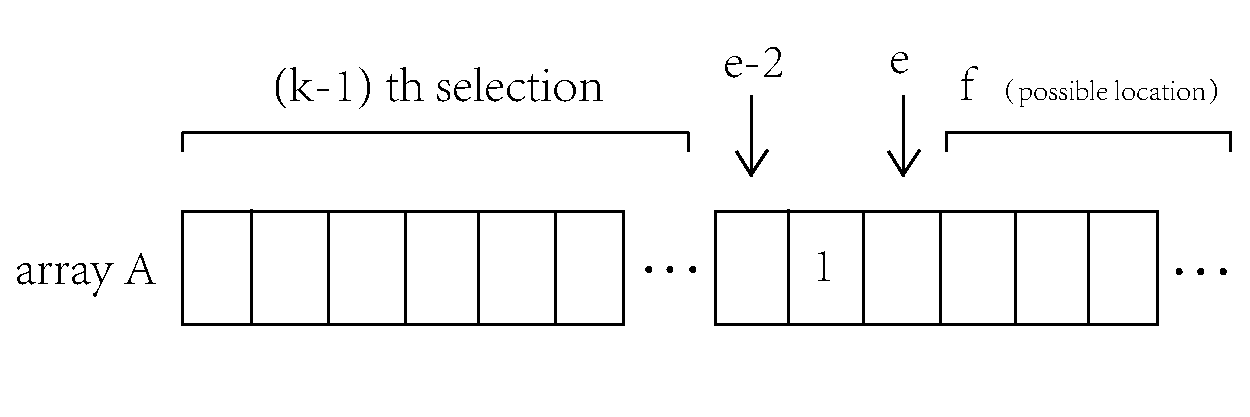
\includegraphics[width=0.63\textwidth]{figures/1_1.pdf}
                \caption{An Illustration of Case 2}\label{1_1}
            \end{figure}
    		\item  \textbf{case 2:} If $e<f$, it means $O$ choose a position $f$ after $G$ chosen $e$. With the greedy algorithm description, we can claim that position $e-1$ must be 1(have a house), and $e-2$ can't exist a hydrant, otherwise position $e$ can't be chosen by $G$. It means that, position $e-1$ have not be covered by any hydrant in (k-1)-th selection. For optimal selection choosing position $f$ after $e$, $e-1$ can't be covered, which have a contradiction with optimal definition, therefore this situation can't exist. 
    		\item  \textbf{case 3:} If $e>f$, greedy algorithm choose a later position than optimal algorithm, we can devide this case into two small one.
    		\begin{itemize}
    			\item []\textbf{key observation:} According to the contradiction in \textbf{case 2}, we can claim in arbitrary intreval [f,m], $G$ choosing positions less than $O$ choosing positions, otherwise, $O$ will have not covered 1(house). 
    			\begin{itemize}
    				\item \textbf{key observation proof:}
    				Assume in the interval [f,m], $G$ choose d positions, and $O$ have chosen no more than d-1 positions. The presupposition $e > f$ means $f\leq e-1$, for greedy algorithm, a chosen position $i$ must have a house at position $i-1$. Therefore, the interval [f,m] have more than d houses, and for these d houses just before chosen position, which mutually at a distance of 3, according to \textbf{Pigeonhole Principle}, the $O$ algorithm can't cover all house, it's a contradiction. 
    			\end{itemize}
    			\begin{figure}[htbp]
                    \centering
                    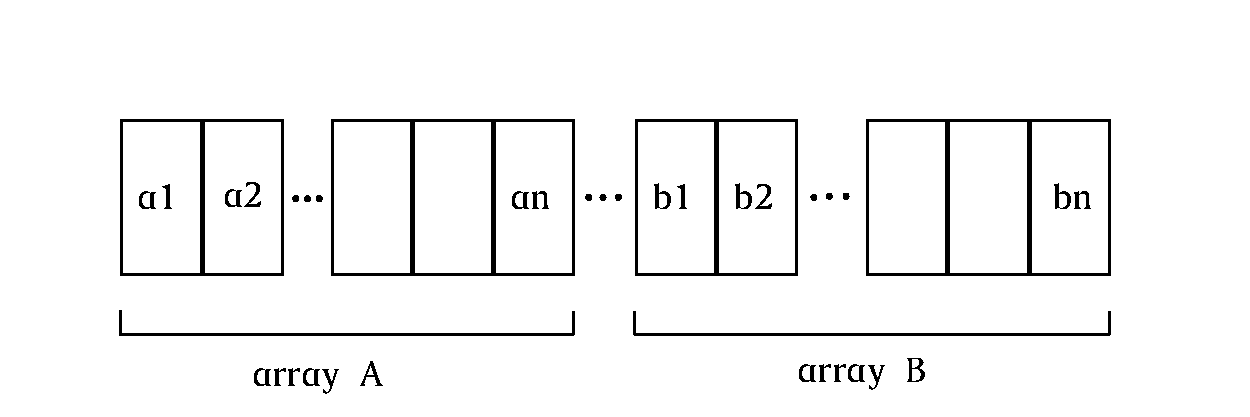
\includegraphics[width=0.63\textwidth]{figures/1_2.pdf}
                    \caption{An Illustration of Case 3 key observation}\label{1_2}
                \end{figure}
    			\item  \textbf{case 3a:} If there exsit r-th selection ($r>k$) before array A ends (street ending), which satisfies that in r-th selection, $G$ and $O$ choose the same postion, which satisfies $Invariant 1$. And according to key observation, $G$ is no worse than $O$ between [k,r].
    			\item  \textbf{case 3b:} If there not exist any same selection position after postion $f$, we can set A[n] as the end element both algorithm have chosen. In that case, according to key observation, $G$ is no worse than $O$ after k-th selection until ending.
    		\end{itemize}
    	\end{itemize}
    \end{itemize}
    As is mentioned above, Greedy-Selection algorithm is no worse than optimal algorithm, and their selection equals when there is noly one optimal solution.
    \end{solution}

    \item
\begin{enumerate}
\item
    Given a set $A$ containing $n$ real numbers, and you are allowed to choose $k$ numbers from $A$. The bigger the sum of the chosen numbers is, the better. What is your algorithm to choose? Prove its correctness using \textbf{Matroid}.\par
\textbf{Remark:} This is a very easy problem. Denote $\mathbf{C}$ be the collection of all subsets of $A$ that contains no more than $k$ elements. Try to prove $(A,\mathbf{C})$ is a matroid.\par
    \begin{proof}\item
    \textbf{Algorithm Description:} We first sort these $k$ numbers with nonincreasing ordering. Then we get the maximum number one by one until we get total $k$ numbers.
    \item\textbf{Pseudo Code:}
    \item
        \begin{minipage}[t]{0.8\textwidth}
        \begin{algorithm}[H]
        \KwIn{An array $A[1 \cdots n]$}
        \KwOut{Set $B$ contains k numbers which have optimal sum}
        \BlankLine
        \caption{Greedy-Selection}
        \label{ALG3}
        \BlankLine
        $Sort\ n\ numbers\ in\ nonincreasing\ ordering\ A[1] \geq A[2] \geq \cdots \geq A[n]$\;
	    $B\leftarrow \emptyset$\;
	    \For{$i\leftarrow 1$ \textbf{to} $k$}{
	        $B\leftarrow B \cup A[i]$\;
	    }
	    $return\ B$\;

        \end{algorithm}
        \end{minipage}
        \hfill
    \item \textbf{Correctness Proof:} Denote $\mathbf{C}$ be the collection of all subsets of $A$ that contains no more than $k$ elements. We first prove system $(A,\mathbf{C})$ satisfies \textbf{Hereditary} and \textbf{Exchange Property}.
    \renewcommand{\qedsymbol}{}
        \begin{itemize}\par
        	\item \textbf{Hereditary:} If $D \subset B$ and $B \in \mathbf{C}$, meaning $D$ is a subset of $A$ which contains no more than $k$ elements. Therefore, $D$ must be an element in subset collection $\mathbf{C}$.
        	\item \textbf{Exchange Property:} Once we choice two element $D, F \in \mathbf{C}$ and $|D| < |F|$, it means $|D|<k$, $\exists x \in F\backslash D$, $D \cup \{x\}$ can be a subset of $A$ which is no more than k. Therefore, $D \cup \{x\} \in \mathbf{C}$.
        \end{itemize}
    \item Now that the problem can be converted into matroid, as its subproblems follow this conversion, this problem can use greedy algorithm (for example, Alg.~\ref{ALG3}) to get one of optimal solution, so our algorithm is correct.
    \end{proof}
\item
Consider that $B_1,B_2 ... B_n$ are $n$ disjoint sets, and let $d_i$ be integers with $0\leq d_{i}\leq |B_{i}|$. Define $\mathbf{C}$ is a collection of set $X$, where $X$ has such property:
$$\forall i\in \{1,2,3 ... n\},  |X\cap B_{i}|\leq d_{i}$$
Prove that $(\cup^{n}_{i=1} B_i,\mathbf{C})$ is a matroid.\par
\textbf{Remark:} You may easily find that the matroid in (a) is a special case of matroid in (b).
    \begin{proof}
    \renewcommand{\qedsymbol}{}\item
       System $(\cup^{n}_{i=1} B_i,\mathbf{C})$ is a matroid \textbf{iff} System $(\cup^{n}_{i=1} B_i,\mathbf{C})$ satisfies \textbf{Hereditary} and \textbf{Exchange Property}.
       \begin{itemize}
           \item \textbf{Hereditary:} If $P \in \mathbf{C}$, which means $\forall i\in \{1,2,3 ... n\},  |P\cap B_{i}|\leq d_{i}$. Then for any subsets P' of P, it's obvious that $|P'\cap B_{i}|\leq |P\cap B_{i}|\leq d_{i}$, P' must be an element of collection $\mathbf{C}$. It says that $P' \subset P,P \in \mathbf{C} \Rightarrow P' \in \mathbf{C}$
           \item \textbf{Exchange Property:} For any elements $P,Q \in \mathbf{C}$ and $|P| < |Q|$. With regard to set $P$, there must exists a group of inequation:
           $$|P\cap B_{1}|\leq d_{1}$$
           $$|P\cap B_{2}|\leq d_{2}$$
           $$\cdots$$
           $$|P\cap B_{k}|< d_{k}$$
           $$\cdots$$
           $$|P\cap B_{n}|\leq d_{n}$$
           $\exists k\in \{1,2,3 ... n\}$, which makes $|P\cap B_{k}|< d_{k}$ (equal mark can't be established in this inequation). Otherwise, any extension will violate constraint equation $$\forall i\in \{1,2,3 ... n\},  |P\cap B_{i}|\leq d_{i}$$ which will lead Q not exists.\item []\item []
           In the other hand, since $|P| < |Q|$ and $Q\in \mathbf{C}$, $Q$ must have an extension element $\epsilon$ in $B_k$ (k-th inequation can't get equal mark established in P's constraint inequations, otherwise which can lead Q not exists as before). Then we can choose this extension $\epsilon$ as $x \in Q\backslash P$, $P \cup \{x\}$ will satisfies the constraint inequations, which means $P \cup \{x\} \in C$.
       \end{itemize}
       In summary, System $(\cup^{n}_{i=1} B_i,\mathbf{C})$ is a matroid.
    \end{proof}


\end{enumerate}
  

    

\end{enumerate}

\vspace{20pt}

\textbf{Remark:} You need to include your .pdf and .tex files in your uploaded .rar or .zip file.

%========================================================================
\end{document}
